% !TeX root = ../praktikum.tex
% !TeX encoding = UTF-8
% !Tex spellcheck = de_DE


Anhand der Messdaten aus der Gleichstrommessung, abgebildet in Graphik \ref{fig:full_range_dc} und \ref{fig:2T_range_dc}, wurde die Dichte der Ladungsträger im 2DEG, sowie deren Beweglichkeit bestimmt.

\subsubsection{Näherung über die Hall-Spannung}
\label{ch:naeherung_hall}

Zunächst wurde die Steigung der Hall-Spannung mittels linearer Regression aus dem klassischen Bereich der Messdaten zwischen \unit[-2]{T} und \unit[2]{T} anhand der Formel $ U_{Hall}=a\cdot B $  
bestimmt:
\begin{equation}
	a=\d{U_{Hall}}{B} = (1869,29 \pm 1,10)\cdot10^{-6} \cdot  \unitfrac{m^2}{s}
\end{equation}

Hieraus ließ sich mit der Formel~\eqref{eq:ladungsdichte_steig} und dem bekannten Strom von $I=\unit[100]{nA}$ die Ladungsträgerdichte des 2DEG berechnen: 
\begin{equation}
	n_s= \frac{I}{e}\left({\niced{U_{Hall}}{B}}\right)^{-1}=( 33.435,1 \pm 19,7) \cdot 10^{10}\cdot \unitfrac{1}{cm^2}
\end{equation}
Mit den Bekannten Maßen der Probe wurde anschließend die Beweglichkeit der Ladungsträger bestimmt. Dies erfolgte anhand der Formel \\
\begin{equation}
	\mu=\frac{1}{n_se}\frac{I}{U_{xx}}\frac{L}{W}
\end{equation}
und mit den Probenmaßen von $L=600\mu m$ für die Länge und
 $B=100\mu m$ für die Breite. \\
\begin{equation}
\mu= \unitfrac{cm^2}{Vs} %TODO: ZAHLENWERTE!
\end{equation}
 
\subsubsection{Näherung über die Shubnikov-de Haas-Oszillation}
\label{ch:naeherung_sdho}

Eine Alternative Möglichkeit, die Ladungsträgerdichte zu berechnen, erfolgt über die Shubnikov-de Haas-Oszillation. Hierzu wurde die Längsspannung über der Probe 
%$U_{Längs}$
 gegen $\unitfrac{1}{B}$ aufgetragen und jedem Minimum der Oszillation ein Füllfaktor $\nu$ zugeordnet. Dies ist in Abbildung~\ref{fig:dc_sdho_ausw} zu sehen. 

Mit der Steigung der Geraden von $A=...$  %TODO: ZAHLENWERTE!
ließ sich analog zur Näherung über die Hallspannung mit Gleichung %TODO: REF! 
die Ladungsträgerdichte bestimmen:
\begin{equation}
n_s= \unitfrac{1}{cm^2}   %TODO: ZAHLENWERTE! 
\end{equation}

So ergibt sich aus Gleichung %TODO: REF! 
für die Beweglichkeit:
\begin{equation}
\mu= \unitfrac{cm^2}{Vs}   %TODO: ZAHLENWERTE! 
\end{equation}
 

\begin{figure}[h]
	\centering
	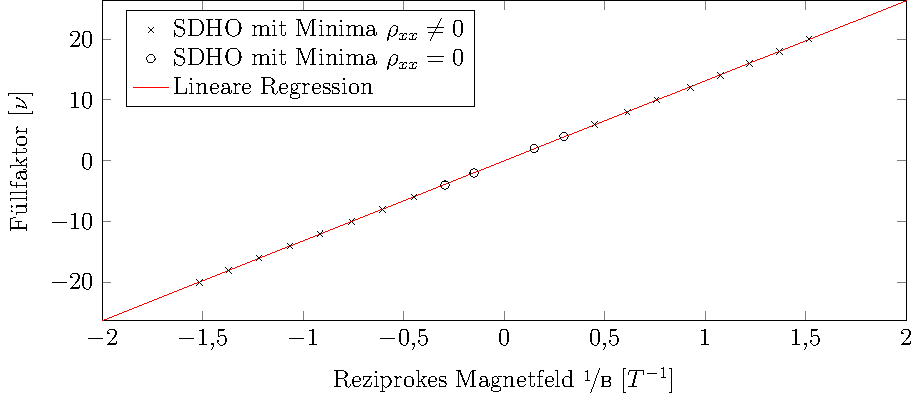
\includegraphics{graphs/dc/auswertung.pdf}
	\caption[Auswertung Füllfaktor Gleichstrommessung]{
		Auswertung Füllfaktor Gleichstrommessung.
	}
	\label{fig:dc_sdho_ausw}
\end{figure}

\begin{equation}
\nu= A\cdot \nicefrac{1}{B}=(13.1462 \pm 0.0190)T \cdot \nicefrac{1}{B}
\end{equation}

In den Graphen \ref{fig:full_range_dc} und \ref{fig:2T_range_dc} fiel eine leichte Asymmetrie der Messkurven auf. Da sich dies in allen folgenden Messungen ebenfalls bemerkbar machte, wurde hier auf einen Fehler an der Probe selbst geschlossen. So ist es zum Beispiel möglich, dass die Kontakte an der Probe zur Messung der Längs- und Hallspannungen unterschiedlich gut an der Probe selbst oder den Messkontakten anliegen. 